\chapter{On the Trento angle convention}

\iffalse
phi1 = angle(v3l,v3h)
phi2 = angle(v3l,v3g)
where if dot(v31,pro > 0,), phi1 =  360 - phi1
if  dot(v31,pro < 0,), phi1 =  phi1 I think check this

v3l = cross(beam,ele) = pe x pe'
v3h = cross(pro,vgs) = pp' x pgamma*
v3g = cross(vgs,pi0) = pgamma* x ppi0
ppi0 = pgamma1+pgamma2

vgs = (-Epx,-Epy, pbeam-df(EPZ) = (-pe'x, -pe'y, pbeam-pe'z) where pbeam = sqrt(beam-me^2)

angle = arccos(costheta(vec1,vec2))
costheta = v1*v2/sqrt(v1*v1*v2*v2)

Thus:
phi = arccos( (v3l dot v3h) / (mag v3l mag v3h) ) 
\fi
phi =    \footnotesize{$\cos^{-1} \left( \frac{ \left(p_{e} \times p_{e'} \right) \cdot \left( p_{p'} \times p_{\gamma^*} \right) }{ \lVert p_{e} \times p_{e'} \rVert \: \lVert p_{p'} \times p_{\gamma^*} \rVert} \right)$}

if dot(pe cross pe', pp') is greater than 0, then do 360 - phi = phi.
If we expand the above out, we get:
-pp'x*ez*ey' + py*ez*ex' is greater than zero
which we can reduce to 
-pp'x*ey' + py*ex' is greater than zero

By inspecting table below, we can see what this really amounts to, is the trento convention saying that we take the angle by measuring counterclockwise from the proton vector to the electron vector.


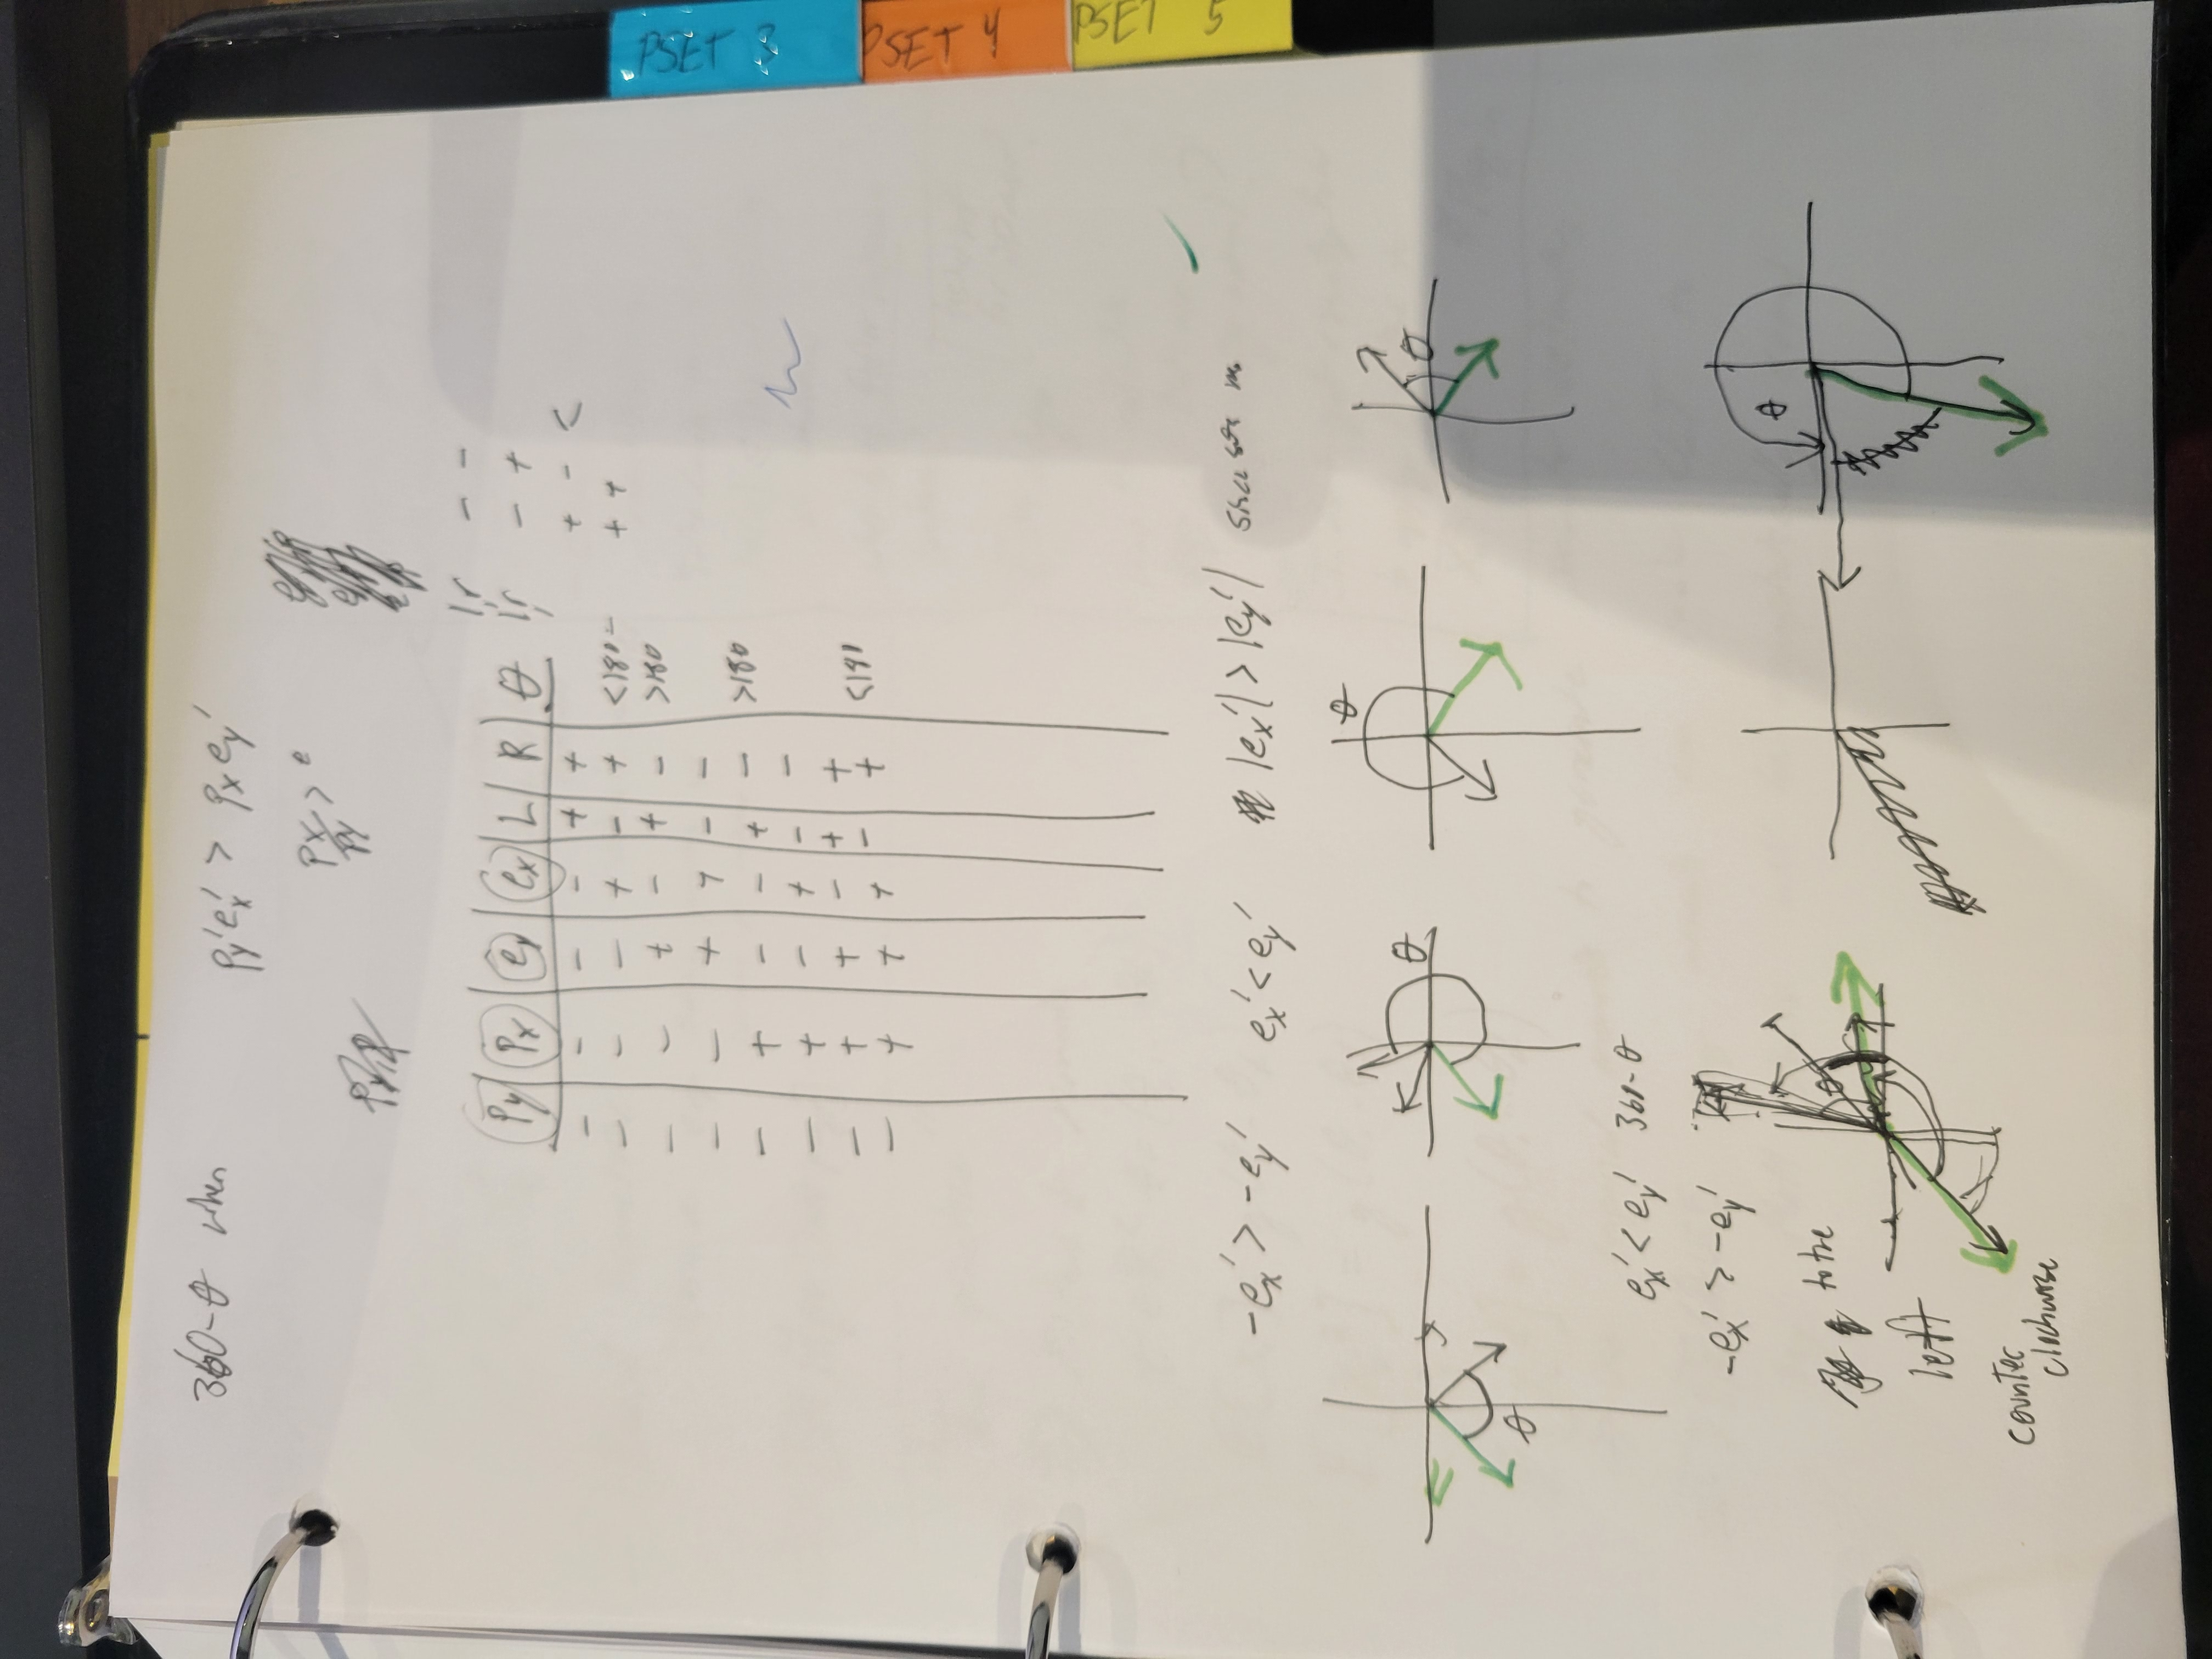
\includegraphics[width=0.9\textwidth]{basics/phi_math_1.jpg}